\documentclass{article}
\usepackage{mainPoly}

\title{Produit scalaire, orthogonalité}
\date{}
\author{Première Spécialité Mathématiques}

\begin{document}
\maketitle

\section{Première définition du produit scalaire}

Lorsque que la notion de vecteur a été définie, l'objectif était d'avoir un objet géométrique capable de se comporter comme un nombre. Ainsi, on a défini en classe de seconde l'\emph{addition}, la \emph{soustraction} de vecteurs, ainsi que la multiplication d'un vecteur par un \emph{scalaire}.

L'objectif est de définir une nouvelle opération sur les vecteurs qui se comporte comme une \emph{multiplication entre deux vecteurs}.

On se place sur le plan.

\begin{tcolorbox}
\begin{definition}
Soit $\vect{u}$ un vecteur. Alors, la norme de $\vect{u}$ (sa \og longueur \fg) est notée $\norm{\vect{u}}$.
\end{definition}
\end{tcolorbox}

\begin{tcolorbox}
\begin{definition}
Soient $\vect{u}$ et $\vect{v}$ deux vecteurs non nuls. On pose $A$, $B$, $C$ trois points du plan tels que $\vect{u} = \vect{AB}$ et $\vect{v} = \vect{AC}$. On note $\widehat{\vect{u},\vect{v}}$ l'angle $\widehat{BAC}$. 
\end{definition}
\end{tcolorbox}
\begin{center}
\begin{tikzpicture}
\coordinate (A) at (0,0);
\coordinate (B) at (15:2);
\coordinate (C) at (80:2.5);

\draw[->] (A) node[left] {$A$} -- (B) node[midway, below] {$\vect{u}$} node[right] {$B$};
\draw[->] (A) -- (C) node[midway, left] {$\vect{v}$} node[above] {$C$};

\draw ($(A)!0.4!(B)$) arc[radius=0.8, start angle=15, end angle=80] node[midway, above right] {$\widehat{\vect{u},\vect{v}}$};
\end{tikzpicture}
\end{center}

\begin{example}
Pour chaque couple de vecteurs $\vect{u}$ et $\vect{v}$ suivants, construire trois points $A$, $B$ et $C$ tels que $\widehat{\vect{u},\vect{v}} = \widehat{BAC}$.

\vspace{0.3cm}
\begin{minipage}{0.25\textwidth}
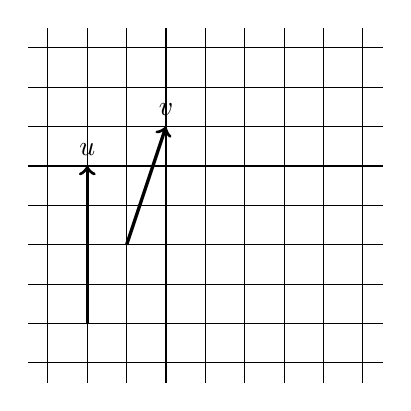
\begin{tikzpicture}
\draw (-0.25,-0.25) grid[step=0.5,color=gray!50] (4.25,4.25);
\draw[->,very thick] (0.5,0.5) -- ++(0,2) node[above] {$\vect{u}$}; 
\draw[->,very thick] (1,1.5) -- ++(0.5,1.5) node[above] {$\vect{v}$}; 
\end{tikzpicture}
\end{minipage}
\hfill
\begin{minipage}{0.25\textwidth}
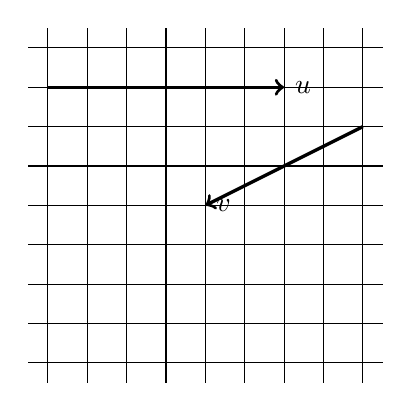
\begin{tikzpicture}
\draw (-0.25,-0.25) grid[step=0.5,color=gray!50] (4.25,4.25);
\draw[->,very thick] (0,3.5) -- ++(3,0) node[right] {$\vect{u}$};
\draw[->,very thick] (4,3) -- ++(-2,-1) node[right] {$\vect{v}$};
\end{tikzpicture}
\end{minipage}
\hfill
\begin{minipage}{0.25\textwidth}
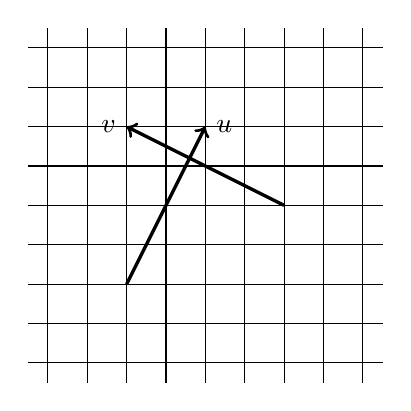
\begin{tikzpicture}
\draw (-0.25,-0.25) grid[step=0.5,color=gray!50] (4.25,4.25);
\draw[->,very thick] (1,1) -- ++(1,2) node[right] {$\vect{u}$};
\draw[->,very thick] (3,2) -- ++(-2,1) node[left] {$\vect{v}$};
\end{tikzpicture}
\end{minipage}
\hfill
\end{example}

\begin{tcolorbox}
\begin{definition}[Produit scalaire]
Soient $\vect{u}$ et $\vect{v}$ deux vecteurs. On appelle \textbf{produit scalaire} de $\vect{u}$ et de $\vect{v}$, noté $\vect{u} \cdot \vect{v}$, le nombre:
\begin{itemize}
\item $0$ si $\vect{u}$ est nul ou $\vect{v}$ est nul.
\item $\norm{\vect{u}} \times \norm{\vect{v}} \times \cos\left(\widehat{\vect{u},\vect{v}}\right)$ dans le cas contraire.
\end{itemize}
\end{definition}    
\end{tcolorbox}



\end{document}